% Options for packages loaded elsewhere
\PassOptionsToPackage{unicode}{hyperref}
\PassOptionsToPackage{hyphens}{url}
\PassOptionsToPackage{dvipsnames,svgnames*,x11names*}{xcolor}
%
\documentclass[
  12pt,
]{article}
\usepackage{amsmath,amssymb}
\usepackage[]{mathptmx}
\usepackage{ifxetex,ifluatex}
\ifnum 0\ifxetex 1\fi\ifluatex 1\fi=0 % if pdftex
  \usepackage[T1]{fontenc}
  \usepackage[utf8]{inputenc}
  \usepackage{textcomp} % provide euro and other symbols
\else % if luatex or xetex
  \usepackage{unicode-math}
  \defaultfontfeatures{Scale=MatchLowercase}
  \defaultfontfeatures[\rmfamily]{Ligatures=TeX,Scale=1}
\fi
% Use upquote if available, for straight quotes in verbatim environments
\IfFileExists{upquote.sty}{\usepackage{upquote}}{}
\IfFileExists{microtype.sty}{% use microtype if available
  \usepackage[]{microtype}
  \UseMicrotypeSet[protrusion]{basicmath} % disable protrusion for tt fonts
}{}
\makeatletter
\@ifundefined{KOMAClassName}{% if non-KOMA class
  \IfFileExists{parskip.sty}{%
    \usepackage{parskip}
  }{% else
    \setlength{\parindent}{0pt}
    \setlength{\parskip}{6pt plus 2pt minus 1pt}}
}{% if KOMA class
  \KOMAoptions{parskip=half}}
\makeatother
\usepackage{xcolor}
\IfFileExists{xurl.sty}{\usepackage{xurl}}{} % add URL line breaks if available
\IfFileExists{bookmark.sty}{\usepackage{bookmark}}{\usepackage{hyperref}}
\hypersetup{
  pdftitle={Age structure and malaria rates in the Legal Amazon: a demographic perspective},
  pdfauthor={Vinícius de Souza Maia; Natália Martins Arruda; Carlos Eduardo Beluzo; Bianca Cechetto Carlos; Luciana Correia Alves},
  pdfkeywords={Sustainable Development Goals (SDGs), Decomposition analysis/methods, Health and morbidity, Applied demography, Age structure, Population ageing, Amazon, Malaria},
  colorlinks=true,
  linkcolor=blue,
  filecolor=Maroon,
  citecolor=Blue,
  urlcolor=Blue,
  pdfcreator={LaTeX via pandoc}}
\urlstyle{same} % disable monospaced font for URLs
\usepackage[margin=1in]{geometry}
\usepackage{longtable,booktabs,array}
\usepackage{calc} % for calculating minipage widths
% Correct order of tables after \paragraph or \subparagraph
\usepackage{etoolbox}
\makeatletter
\patchcmd\longtable{\par}{\if@noskipsec\mbox{}\fi\par}{}{}
\makeatother
% Allow footnotes in longtable head/foot
\IfFileExists{footnotehyper.sty}{\usepackage{footnotehyper}}{\usepackage{footnote}}
\makesavenoteenv{longtable}
\usepackage{graphicx}
\makeatletter
\def\maxwidth{\ifdim\Gin@nat@width>\linewidth\linewidth\else\Gin@nat@width\fi}
\def\maxheight{\ifdim\Gin@nat@height>\textheight\textheight\else\Gin@nat@height\fi}
\makeatother
% Scale images if necessary, so that they will not overflow the page
% margins by default, and it is still possible to overwrite the defaults
% using explicit options in \includegraphics[width, height, ...]{}
\setkeys{Gin}{width=\maxwidth,height=\maxheight,keepaspectratio}
% Set default figure placement to htbp
\makeatletter
\def\fps@figure{htbp}
\makeatother
\setlength{\emergencystretch}{3em} % prevent overfull lines
\providecommand{\tightlist}{%
  \setlength{\itemsep}{0pt}\setlength{\parskip}{0pt}}
\setcounter{secnumdepth}{-\maxdimen} % remove section numbering
\usepackage{booktabs}
\usepackage{longtable}
\usepackage{array}
\usepackage{multirow}
\usepackage{wrapfig}
\usepackage{float}
\usepackage{colortbl}
\usepackage{pdflscape}
\usepackage{tabu}
\usepackage{threeparttable}
\usepackage{threeparttablex}
\usepackage[normalem]{ulem}
\usepackage{makecell}
\usepackage{xcolor}
\ifluatex
  \usepackage{selnolig}  % disable illegal ligatures
\fi
\usepackage[numbers, round, super]{natbib}
\bibliographystyle{unsrtnat}

\title{Age structure and malaria rates in the Legal Amazon: a demographic perspective}
\author{Vinícius de Souza Maia \and Natália Martins Arruda \and Carlos Eduardo Beluzo \and Bianca Cechetto Carlos \and Luciana Correia Alves}
\date{}

\begin{document}
\maketitle
\begin{abstract}
Despite advances in reducing the burden and mortality of malaria in recent decades, the disease remains relevant for population health in the Legal Amazon region of Brazil. At the same time that rates have been decreasing from 18.4 cases per 1000 people to only 5.4 cases per 1000, the brazilian population has experienced rapid changes age structure. We combine data from National Household Surveys and the Malaria Epidemiological Surveillance System to estimate the contribution of age to malaria rate schedules, using visualizations and decomposition to compare the years 2007 and 2019 for nine states in the Legal Amazon. Our preliminary findings show that although malaria rates have fallen considerably from 2007 to 2019, changes in population structure have non-negligible contribution to changes in malaria rate schedules, especially since states have had malaria rate reductions and population structure changes of varying intensity. We tentatively conclude that the contribution of age structure to malaria rate schedules will tend to increase as further reductions in rates become more challenging in the next few years and trends in fertility and mortality in the country will probably accelerate population aging.
\end{abstract}

\hypertarget{introduction}{%
\subsection{Introduction}\label{introduction}}

Worldwide, malaria is major health issue, with over 200 million cases every year and over 400,000 deaths each year \citep{WorldMalariaReport}. Despite the progress made in the previous decades, it continues to be a common disease in the Legal Amazon region of Brazil, where 157 thousand cases were reported in 2019 and another 60 thousand in the first half of 2020 \citep{saudeBoletimEpidemiologicoMalaria2020}. For this reason, one of the goals of National Malaria Control Program (NCMP) is the eradication of the disease, with current goals of eliminating \emph{P. falciparum} malaria until 2030.

However, as the country has reduced disease incidence rapidly in the preceding decades, the disease has become more focal and heterogeneously distributed in the territory \citep{lanaTopQuantifyingUnequal2021} and further reductions in malaria rates will probably become more challenging\citep{ferreiraChallengesMalariaElimination2016} to achieve with wide-ranging strategies, requiring tailored, local approaches. This is especially relevant considering the complex nature of malaria risk, which involves ecological, demographic, socioeconomic and institutional factors complexly intertwined \citep{worldhealthorganizationGlobalTechnicalStrategy2015}.

From a demographic perspective, these successes in malaria control happen at a time where Brazil is undergoing rapid population aging \citep{camaranoPopulacaoBrasileiraSeus2014} and also an expansion of education access. This is relevant for malaria epidemiology because certain age and education profiles tend to show higher levels of disease incidence \citep{bezerraChangesMalariaPatterns2020, corderStatisticalModelingSurveillance2019}, particularly in the Brazilian case, where the pattern has shifted from younger towards adult, working-age populations. So, it is reasonable to ask if demographic change has had an effect on the rate schedules of malaria and, if so, to what extent.

In summary, the goal of this study is to compare the age structure of the population afflicted with malaria in Brazil in the years 2007 and 2019 and to estimate the contribution of demographic and education changes to changes in malaria rates schedules in the context of falling malaria incidence rates.

\hypertarget{methods}{%
\subsection{Methods}\label{methods}}

Data on population estimates for states in the LA region was obtained from the National Household Sample Survey (PNAD) for 2007 and the Continuous National Household Sample Survey (PNADC) for 2019. Data on number of cases by age and state was obtained from the Malaria Epidemiological Surveillance System (SIVEP Malaria), maintained by the Ministry of Health.

The study area is the Legal Amazon, a group of nine Brazilian States that contain, in full or in part, the amazon rainforest biome and are, therefore, required by the Constitution to help preserve it. It is composed by the States of Acre (AC), Amapá (AP), Amazonas (AM), Maranhão (MA), Mato Grosso (MT), Pará (PA), Tocantins (TO), Rondônia (RO) and Roraima (RR) and is located in the Northwestern part of Brazil, bordering several countries in South America.

We define a malaria case as a positive slide test that corresponds to a new infection, by discarding cases that were reported as ``cure verification slides'' happening in one of the states in the Legal Amazon in the year 2007 or 2019. The study population is comprised of the estimated population of these states according to the National Institute for Geography and Statistics (IBGE). The malaria rate is the ratio between the number of cases in the given year divided by the estimated midyear population.

We used data visualizations to compare the age structures of malaria cases for both periods and decomposition \citep{prestonDemographyMeasuringModeling2000} to estimate the contribution of age structure to malaria rate schedules.

\hypertarget{results}{%
\subsection{Results}\label{results}}

\begin{figure}
\centering
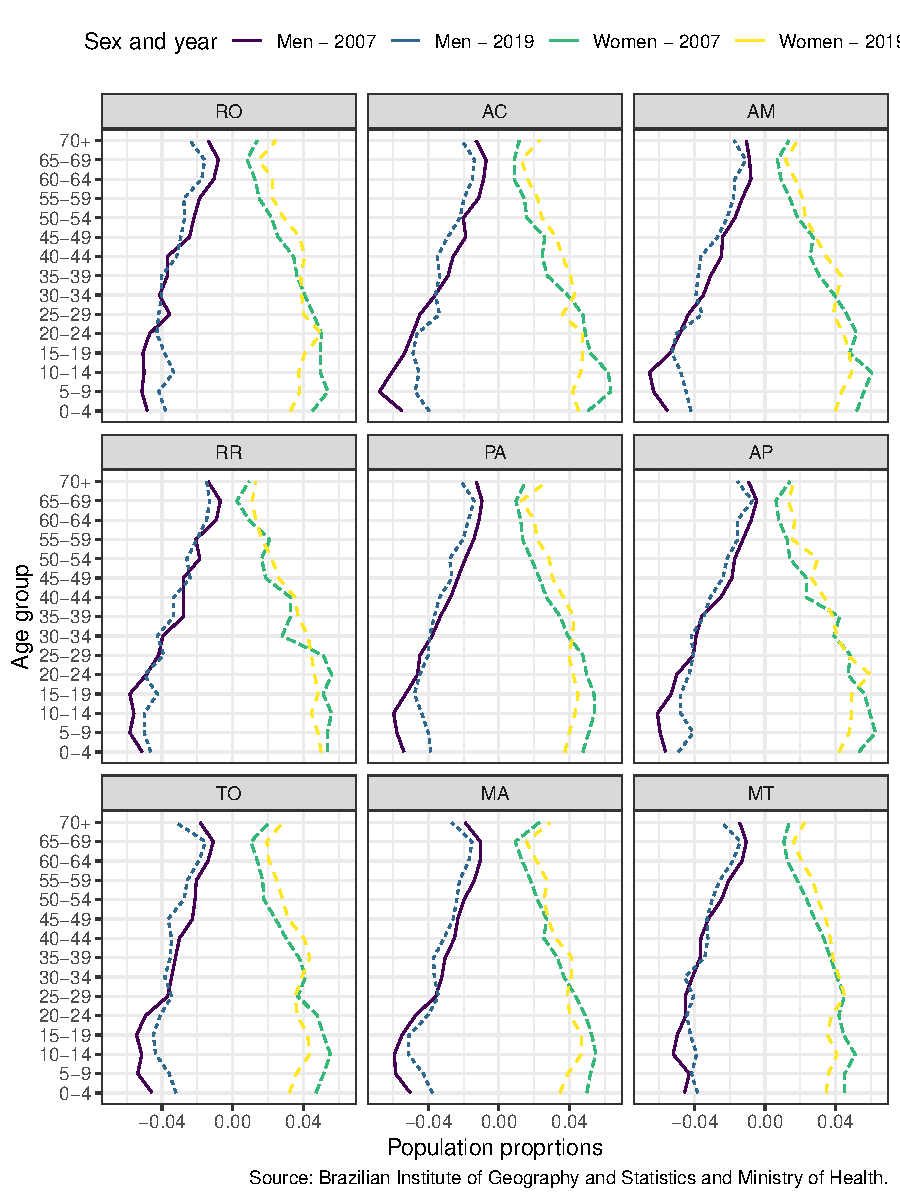
\includegraphics{piramide.pdf}
\caption{\label{fig:piramide}Age and sex structure by State in the Legal Amazon in 2007 and 2019}
\end{figure}

The population age structure for all nine states can be seen in figure \ref{fig:piramide}. These results show that falling fertility can be seen in all states in LA. Even if the effects are not very pronounced in Roraima and Mato Grosso. The population up to 20 years old is smaller in proportion than it was 14 years ago, and the relative contribution of adults over 30 is increasing.

\begin{figure}
\centering
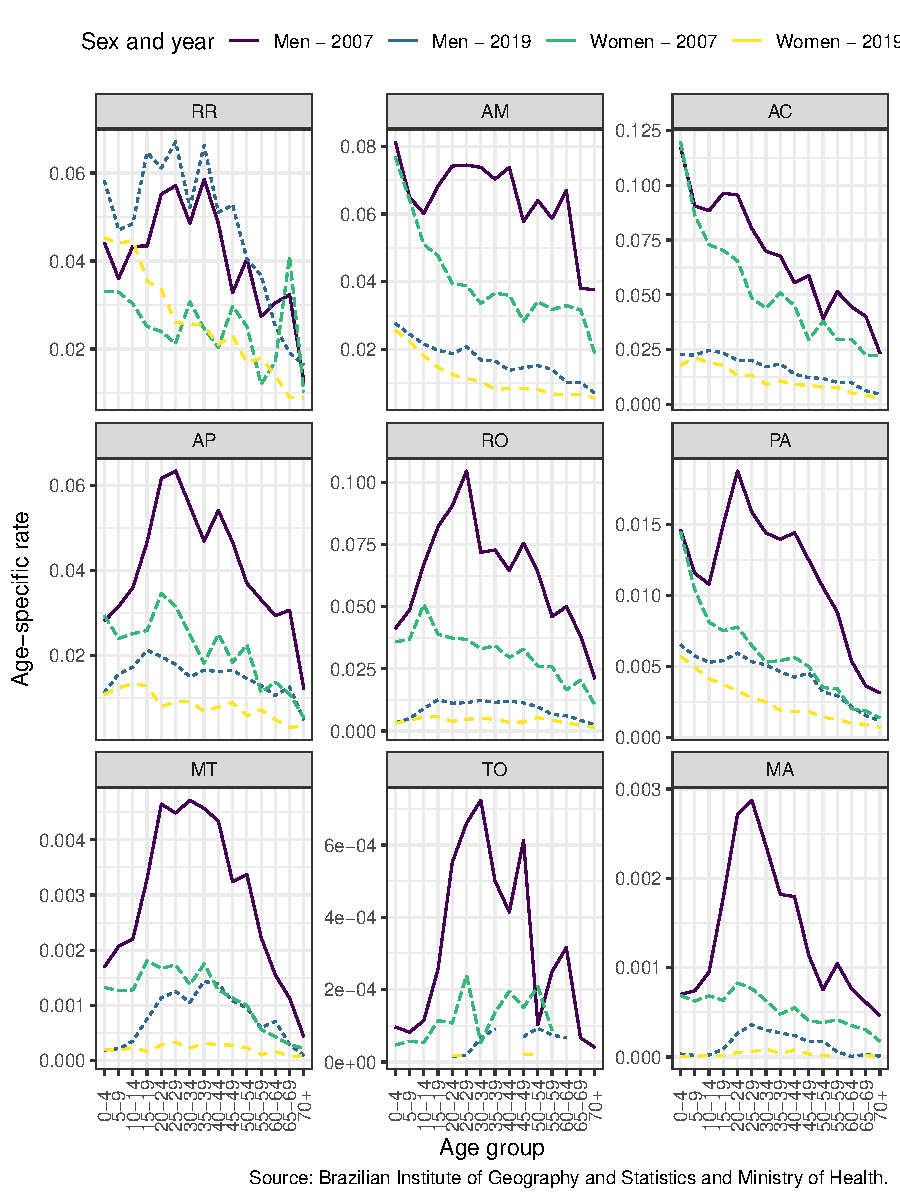
\includegraphics{taxa-especifica-uf.pdf}
\caption{\label{fig:tx-malaria}Age specific malaria rate by sex and State in Legal Amazon in 2007 and 2019}
\end{figure}

The age distribution of malaria cases in 2007 and 2019 can be seen in figure \ref{fig:tx-malaria}. With the exception of Roraima (RR), where the levels of malaria infection have not changed substantially between the two comparison years, all other states have shown marked reductions in the overall rates of infection. With these also came a reduction in the sex difference between rates, which can be seen by the reduction of the gap between the lines for men and women. Another relevant feature is that in most states the proportion younger than 15 has been reduced in relation to the working age population, which can be seen by a decrease of the relative slope of the line for young in relation to working age people, becoming positive for young people in states where the rates are lowest.

\begin{table}[!h]

\caption{\label{tab:decomp}Age and rate decomposition by State in the Legal Amazon, 2007 and 2019}
\centering
\begin{tabular}[t]{>{\raggedright\arraybackslash}p{8em}>{\centering\arraybackslash}p{6em}>{\centering\arraybackslash}p{6em}>{\centering\arraybackslash}p{6em}>{\centering\arraybackslash}p{6em}}
\toprule
State & Age & Rate & Age Contribution & Rate Contribution\\
\midrule
\addlinespace[0.3em]
\multicolumn{5}{l}{\textbf{Men}}\\
\hspace{1em}RO & 0.0006 & 0.0284 & 1.9\% & 98.1\%\\
\hspace{1em}AC & 0.0025 & 0.0295 & 7.7\% & 92.3\%\\
\hspace{1em}AM & 0.0006 & 0.0243 & 2.2\% & 97.8\%\\
\hspace{1em}RR & 0.0006 & -0.0044 & -16.8\% & 116.8\%\\
\hspace{1em}PA & 0.0003 & 0.0040 & 6.5\% & 93.5\%\\
\hspace{1em}AP & 0.0005 & 0.0133 & 3.8\% & 96.2\%\\
\hspace{1em}TO & 0.0000 & 0.0001 & -5.5\% & 105.5\%\\
\hspace{1em}MA & 0.0000 & 0.0007 & -0.3\% & 100.3\%\\
\hspace{1em}MT & 0.0000 & 0.0012 & 2.5\% & 97.5\%\\
\addlinespace[0.3em]
\multicolumn{5}{l}{\textbf{Women}}\\
\hspace{1em}RO & 0.0004 & 0.0150 & 2.8\% & 97.2\%\\
\hspace{1em}AC & 0.0012 & 0.0241 & 4.9\% & 95.1\%\\
\hspace{1em}AM & 0.0009 & 0.0154 & 5.3\% & 94.7\%\\
\hspace{1em}RR & 0.0002 & -0.0026 & -6.3\% & 106.3\%\\
\hspace{1em}PA & 0.0002 & 0.0019 & 9.9\% & 90.1\%\\
\hspace{1em}AP & 0.0000 & 0.0077 & 0.3\% & 99.7\%\\
\hspace{1em}TO & 0.0000 & 0.0000 & -6.0\% & 106.0\%\\
\hspace{1em}MA & 0.0000 & 0.0003 & 3.5\% & 96.5\%\\
\hspace{1em}MT & 0.0000 & 0.0005 & 2.6\% & 97.4\%\\
\bottomrule
\multicolumn{5}{l}{\rule{0pt}{1em}\textit{Source: } Brazilian Institute of Geography and Statistics and Ministry of Health.}\\
\end{tabular}
\end{table}

The results of age decomposition by state can be seen in table \ref{tab:decomp}. The contribution of age structure change to malaria rate schedules is very modest in most states. For men for instance, Roraima, Tocantins and Maranhão show no contribution at all; Rondônia, Amapá and Mato Grosso, less than 2.5\%; and Amapá, Pará and Acre had 3.8, 6.5 and 7.7\% respectively. For women, Roraima and Tocantins showed no contribution; Rondônia, Maranhão and Mato Grosso were below 3.5\%; while Acre, Amazonas and Pará showed slightly larger contributions of 4.9, 5.3 and 9.9\%, respectively.

\hypertarget{discussion-and-conclusions}{%
\subsection{Discussion and conclusions}\label{discussion-and-conclusions}}

At first glance, the small proportions of age contribution to changes in rates would seem negligible, however, they must be considered in light of the enormous reduction in malaria incidence observed over the period. Rates decreased on average 67\%, with states like Rondônia, Tocantins and Maranhão reducing their rates by nearly 90\%. In a scenario such as this one, the mere existence of age structure contributions is remarkable.

Moreover, the trends for the future are the most relevant aspect of this analysis. Currently, the NMCP is pursuing \emph{P. falciparum} malaria elimination and continuing efforts to reduce the overall burden, but further reductions in the rates will be more challenging \citep{ferreiraChallengesMalariaElimination2016, meloEvaluationMalariaElimination2020}. At the same time, current trends in declining fertility and longevity improvements -- however timid they may be will probably accelerate the process of population aging. As a result of this, it is likely that future changes in the age distribution of malaria cases will become more and more influenced by changes in age structure.

In summary, as the country makes progress in the struggle against malaria, the relevance of the demographic perspective increases, both because the disease becomes more localized and heterogeneous \citep{lanaTopQuantifyingUnequal2021}, but also because the structure of the population at risk is changing as well. We hope that future studies can take this dimension into consideration, since population vulnerability is already recognized as one of the determinants of malaria risk.

  \bibliography{references.bib}

\end{document}
